\section{Teilkonzepte}
In diesem Abschnitt werden die Teilkonzepte der evaluierten Lösungsvariante \glqq Frosch\grqq{} beschrieben. Es wurden Konzepte zu den einzelnen Funktionen erstellt. Abschliessend wird das Zusammenspiel der Teilkonzepte anhand eines Blockschaltbild erklärt.

\subsection{Treppensteigen}

\subsubsection{Funktionsprinzip}
Für das Treppensteigen wurde die Variante "Frosch" evaluiert. Der Grundkörper des Gerätes, in dem Antriebe, Steuerung, Energieversorgung und Orientierungskomponenten enthalten sind, wird auf beiden Seiten mit jeweils einem Standfuss und einer Verbindungsleiste erweitert. Von der Drehachse 1 zur Drehachse 2 wird ein Zahnriemen gespannt. Mit diesen zusätzlichen Elementen soll die Treppe bestiegen werden.

\image
 {img/Skizze Drehachsen}
 {Drehachsen}

Eine Treppenstufe soll mit zwei Hubbewegungen erklommen werden. In einer ersten Hubbewegung bleiben die Standfüsse auf der letzten Stufe und der Grundkörper wird auf die nächste Stufe gehoben. Bei dieser Bewegung soll der Grundkörper horizontal gehalten werden.

\image
 {img/Treppensteigen/1. Hubbewegung Skizze}
 {1. Hubbewegung}

Bei der zweiten Hubbewegung müssen die Standfüsse auf die nächste Treppenstufe, zurück an die Seiten des Grundkörpers geholt werden.

\image
 {img/Treppensteigen/2. Hubbewegung Skizze}
 {2. Hubbewegung}

\subsubsection{Funktionen der Komponenten}
Die Verbindungsleisten sind über eine Welle (Welle 1) mit dem Grundkörper verbunden (Drehachse 1). Die Verbindungsleisten sind fest auf der ersten Welle fixiert, sodass bei einer Drehung der Welle sich die Verbindungsleisten um den gleichen Winkel drehen. Das Antriebsrad des Zahnriementriebes ist lose auf der ersten Welle montiert, sodass die Drehbewegungen der Welle und des Antriebsrads des Zahnriemens unabhängig sind.

Die Verbindungsleisten sind mit den Standfüssen bei der zweiten Drehachse verbunden. Diese zweite Drehachse ist nicht eine Drehachse, sondern auf beiden Seiten eine Drehachse für sich selbst. Sie sind aber immer gleich ausgerichtet und werden als eine Drehachse betrachtet (Drehachse 2). Die Standfüsse sind mit den Verbindungsleisten über eine kleine, kurze Welle (Welle 2) verbunden. Diese zweite Welle ist auf beiden Seiten jeweils einmal vorhanden. 

Bei der zweiten Drehachse muss auf beiden Seiten ein Moment aufgebracht werden für die erste Hubbewegung, damit sich die Standfüsse und Verbindungsleisten gegeneinander bei der zweiten Drehachse verdrehen und so der Grundkörper nach oben gehoben wird. Das Moment bei den zweiten Drehachsen kann nicht direkt mit einzelnen, zwei an die Wellen gekoppelten Motoren angetrieben werden, da die Motoren bei den Hubbewegungen im Weg wären, wenn sie an den Innenseiten angebracht würden oder die Kabel des Motors wären im Weg bei einer Aussenmontur. Aus diesem Grund muss das Moment für die erste Hubbewegung von der ersten Welle auf die kleinen, kurzen Wellen auf beiden Seiten übertragen werden. Für diese Übertragung des Drehmomentes mit einem grossen Achsabstand eignen sich Zugmittelgetriebe wie Ketten-, Riementriebe. Da das Gewicht nicht zu gross werden soll, kommen Ketten nicht in Frage. Da das Drehmoment in einem gewissen Verhältnis und ohne Schlupf übertragen werden soll, eignet sich ein Zahnriemen am besten. Der Zahnriemen soll das Moment 1:1 übertragen, was dazu führt, dass beide Zahnriemenräder die gleiche Anzahl Zähne haben und somit auch gleich gross sind. Bei der zweiten Welle sind die Standfüsse mit dem Abtriebs Rad des Zahnriementriebes gekoppelt und machen so die gleichen Drehbewegungen. Weiter sind bei der zweiten Drehachse die Standfüsse nicht mit den Verbindungsleisten gekoppelt, da sie sich zueinander verdrehen müssen, um die Hubbewegungen auszuführen. 

Für die erste Hubbewegung wird an den Antriebszahnriemenrädern ein Moment eingeleitet. Die Antriebszahnriemenräder sollen je mit einem Zahnrad verbunden werden. Mit einer Übersetzung soll ein erster Elektrogetriebemotor diese Antriebszahnriemenräder antrieben. Um den Grundkörper bei der ersten Hubbewegung horizontal halten zu können soll auf der ersten Welle ein Zahnrad angebracht werden, um mit einem zweiten Elektrogetriebemotor das Moment der Gewichtskraft des Grundkörpers auszugleichen.

Bei der zweiten Hubbewegung wird die Drehung der Standfüsse bei der zweiten Drehachse mit dem ersten Motor kontrolliert. Die Drehung der Verbindungsleisten bei der ersten Drehachse wird vom zweiten Motor angetrieben. Mit diesem Aufbau ist es möglich die Standfüsse einzeln zu verdrehen. Somit kann das nötige Drehmoment verkleinert werden, wenn bei der zweiten Hubbewegung die Standfüsse nicht horizontal gehalten werden.

TODO Bilder der Komponenten

\subsubsection{Erste Abmasse}

Anhand der vorgegebenen Treppe wurden erste Massabschätzungen gemacht. Dabei wurde die Tritthöhe und die Tritttiefe berücksichtigt.

\image
 {img/Erste Abmasse}
 {Erste Abmasse}

\subsubsection{Standsicherheit}

Mit den ersten Massabschätzungen wurde eine erste Standsicherheitsbetrachtung bei den zwei Hubbewegungen gemacht. Dabei wurde das Wunschgewicht, dass in der Anforderungsliste definiert wurde verwendet. Die Standfüsse und die Verbindungsleisten sollen aus Aluminium mit einer Dichte\footnote{https://de.wikipedia.org/wiki/Aluminium} von 2.7 g/cm$^{3}$ sein. Ihr Gewicht wurde mit den ersten Massabschätzungen berechnet.

\newpage

\textbf{Berechnung Masse Standfüsse:}\\

Material: Aluminium

Dicke t: 5 mm

{\rho}$_{Aluminium}$ = 2.7 g/cm$^{3}$\\

V$_{1 Standfuss}$ = a * b * t = 280 mm * 80 mm * 5mm = 112 cm$^{3}$

m$_{1 Standfuss}$ = V$_{1 Standfuss}$ * \rho$_{Aluminium}$ = 112 cm$^{3}$ * 2.7 g/cm$^{3}$ = 0.3 kg\\

m$_{2 Standfuesse}$= 2 * m$_{1 Standfuss}$ = 0.6 kg\\
\\

\textbf{Berechnung Masse Verbindungsleisten:}\\

Material: Aluminium

Dicke t: 5 mm

\rho$_{Aluminium}$ = 2.7 g/cm$^{3}$\\

V$_{1 Verbindungsleiste}$ = a * b * t = 280 mm * 50 mm * 5mm = 70 cm$^{3}$

m$_{1 Verbindungsleiste}$ = V$_{1 Verbindungsleiste}$ * \rho$_{Aluminium}$ = 70 cm$^{3}$ * 2.7 g/cm$^{3}$ = 0.2 kg\\

m$_{2 Verbindungsleisten}$= 2 * m$_{1 Verbindungsleiste}$ = 0.4 kg

\newpage

\textbf{1.Hubbewegung:}\\

m$_{ges}$ = 3kg

m$_{Grundkoerper}$ = 2 kg

m$_{Standfuesse}$ = 0.6 kg

m$_{Verbindungsleisten}$ = 0.4 kg\\

\image
 {img/Standsicherheit 1.Hub.png}
 {Skizze Standsicherheit bei der 1. Hubbewegung}\\

Standsicherheit ist bis {\alpha} = 90$^\circ$ gegeben.

Für {\alpha} = 90$^\circ$ gilt:\\

M$_{Stand}$ = F$_{GS}$ * 140 mm + F$_{GL}$ * 40 mm

            = g (m$_{Standfuesse}$ * 140 mm + m$_{Verbindungsleisten}$ * 40 mm)
            
            = 9.81 m/s$^{2}$ (0.6 kg * 140 mm + 0.4 kg * 40 mm) = 0.9 Nm\\

M$_{Kipp}$  = F$_{GG}$ * 10 mm

            = g (m$_{Grundkoerper}$ * 10 mm)
            
            = 9.81 m/s$^{2}$ (2 kg * 10 mm) = 0.2 Nm\\
            
M$_{Stand}$ > M$_{Kipp}$\\
\\

Für {\alpha} > 90$^\circ$ gilt:\\

\begin{center}

F$_{GS}$ * 140 + F$_{GL}$ (40 - x) = (50 + 2x - 40) ; wenn x < 40

m$_{S}$ * g * 140 + m$_{V}$ * g (40 - x) = m$_{G}$ * g (10 +2x)

m$_{S}$ * 140 + m$_{V}$ * 40 - m$_{V}$ * x = m$_{G}$ * 10 + m$_{G}$ * 2x

(2 * m$_{G}$ + m$_{V}$) x = m$_{S}$ * 140 + m$_{V}$ * 40 - m$_{G}$ * 10

x = (m$_{S}$ * 140 + m$_{V}$ * 40 - m$_{G}$ * 10) / (2 * m$_{G}$ + m$_{V}$)

x = 18.2 mm (erfüllt x < 40 mm)

\end{center}

{\beta} = \arcsin{(18.2 mm / 115 mm)} = 9.1$^\circ$

{\phi} = 90$^\circ$ + {\beta} = 90$^\circ$ + 9.1$^\circ$ = 99.1$^\circ$\\

Bei der ersten Hubbewegung ist die Standsicherheit bis {\phi} = 99.1$^\circ$ gegeben.\\
\\

\textbf{2.Hubbewegung:}\\

\image
 {img/Standsicherheit 2.Hub.png}
 {Skizze Standsicherheit bei der 2. Hubbewegung}

Wenn die Standfüsse bei der 2.Hubbewegunng waagrecht gehalten werden, ist die kritische Stelle der Hubbewegung, wenn die Standfüsse und die Verbindungsleisten in einer Linie mit dem Drehpunkt des Grundkörpers sind.\\

In diesem Fall gilt:\\

M$_{Stand}$ = F$_{GG}$ * 100 mm 

            = g * m$_{Grundkoerper}$ * 100 mm
            
            = 9.81 m/s$^{2}$ * 2 kg * 100 mm
            
            = 1962 Nmm\\

M$_{Kipp}$  = F$_{GS}$ (230 mm + 100 mm - 50 mm) + F$_{GL}$ (115 mm - 50             mm)

            = g (m$_{Standfuesse}$ * 280 mm + m$_{Verbindungsleisten}$ * 65 mm)
            
            = 9.81 m/s$^{2}$ (0.6 kg * 280 mm + 0.4 kg * 65 mm)
            
            = 1903 Nmm\\
            
M$_{Stand}$ > M$_{Kipp}$\\
\\

\subsubsection{1. Hubbewegung Analyse}

Mit den ersten Massabschätzungen und der ersten Platziervorstellung auf dem aktuellen Treppentritt wurde berechnet, ob der Grundkörper bei der erste Hubbewegung mit der Kante des des nächsten Treppentrittes kollidert oder nicht. Es wurde auch berechnet, auf welcher Höhe über dem nächsten Treppentritt und wie weit über der Kante des nächsten Trittes sich der Grundkörper beim kritischen Kippwinkel befindet.

\image
 {img/Platzierung.png}
 {Skizze Platzierung auf aktueller Treppenstufe vor 1. Hubbewegung}

Beim Start der 1. Hubbewegung ist Punkt A 140 mm in X-Richtung vom nächsten Tritt entfernt.\\

Der Drehpunkt B ist in X-Richtung 60 mm vom nächsten Tritt entfernt.

\image
 {img/Analyse 1.png}
 {Skizze kritischer Kippwinkel erreicht}

Wo befindet sich Punkt A, wenn der kritische Kippwinkel \alpha$_{1}$ = 99.1$^\circ$ erreicht ist?

l = 150 mm + 230 mm * sin(\alpha$_{1}$ - 90$^\circ$) = 186. 4 mm

Punkt A in X-Richtung über nächster Trittkante = 186.4 mm - 60 mm = 126.4 mm\\

h = 230 mm * cos(\alpha$_{1}$ - 90$^\circ$) = 227.1 mm

Punkt A in Y-Richtung über nächster Trittkante = 227.1 mm - 200 mm = 27.1 mm\\
\\

Wenn Punkt A in X-Richtung auf gleicher Höhe wie die nächste Trittkante ist, welchen Abstand hat dann Punkt A in Y-Richtung?\\

\image
 {img/Analyse 2.png}
 {Skizze Punkt A in X-Richtung auf Höhe der nächsten Trittkante}

l$_{2}$ = 60 mm

\alpha$_{2}$ = arccos((150 mm - l$_{2}$) / 230 mm) = 67$^\circ$

h$_{2}$ = 230 mm * sin(\alpha$_{2}$)  = 211.7 mm

Punkt A in Y-Richtung über nächster Trittkante wenn Punkt A in X-Richtunng auf gleicher Höhen wie dien nächste Trittkante = 211.7 mm - 200 mm = 11.7 mm\\


\subsubsection{Benötigte Momente}

Die Momente, die gebraucht werden, konnten mit den ersten Gewichts- und Massabschätzungen berechnet werden und dienen als Motorenauswahl Grundlage.

TODO Bild Drehachsen

\textbf{Momente bei den Hubbewegungen:}

\textbf{1.Hubbewegung:}

Drehachse 1: Moment zu horizontalen Halten des Grundkörpers

M$_{Achse 1}$ = F$_{GG}$ * 0.06 m

= m$_{GG}$ * g * 0.06 m

= 2 kg * 9.81 m/s$^{2}$ * 0.06 m

= 1.2 Nm\\

Drehachse 2: grösstes Moment am Anfang, in Ausgagsstellung

M$_{Achse 2}$ = F$_{GL}$ * 0.115 m + F$_{GG}$ * 0.23 m

= g(m$_{GL}$ * 0.115 m + m$_{GG}$ * 0.23 m

= 9.81 m/s$^{2}$(0.4 kg * 0.115 m + 2 kg * 0.23 m)

= 5 Nm\\

\textbf{2.Hubbewegung:}

Drehachse 1: grösstes Moment, wenn alle Teile horizontal

M$_{Achse 1}$ = F$_{GS}$ * 0.33 m + F$_{GL}$ * 0.115 m

= g(m$_{GS}$ * 0.33 m + m$_{GL}$ * 0.115 m)

= 9.81 m/s$^{2}$(0.6 kg * 0.33 m + 0.4 kg * 0.115 m)

= 2.4 Nm\\

Drehachse 2: grösstes Moment, wenn Standfüsse horizontal

M$_{Achse 2}$ = F$_{GS}$ * 0.1 m

= m$_{GS}$ * g * 0.1 m

= 0.6 kg * 9.81 m/s$^{2}$ * 0.1 m

= 0.6 Nm\\

Motor 1 liefert das Moment, das in der 1. Drehachse wirkt und Motor 2 liefert das Moment, das in der 2. Drehachse wirkt.\\
\\
M$_{erforderlich}$ Motor 1: 5 Nm\\

M$_{erforderlich}$ Motor 2: 2.2 Nm


\subsection{Elektrotechnisches Konzept}
\subsubsection{Auslegung Elektromotoren}
Der erste Motor benötigt gemäss Berechnungen ein maximales Drehmoment von 3.9 Nm. Dazu passt der Getriebemotor Modelcraft IG320516-41C01 von conrad \cite{Getriebemotor1}. Dieser liefert ein maximales Drehmoment von 4.2 Nm. 
Der zweite Motor benötigt gemäss Berechnungen ein maximales Drehmoment von 2.2 Nm. Dazu passt der Getriebemotor Modelcraft RB350600-0A101R ebenfalls von conrad \cite{Getriebemotor2}. Dieser liefert ein maximales Drehmoment von 3.2 Nm.

\subsubsection{Sensorik für die Bewegungen}
Die Bewegungen werden durch Elektrogetriebemotoren umgesetzt. Damit die Steuerung die Bewegungen autonom ausführen kann, benötigt die Steuerung Rückmeldungen, in welcher Position sich der Grundkörper und die Standfüsse befinden. Dies soll mittels Tastsensoren realisiert werden.

\begin{figure}[h]
  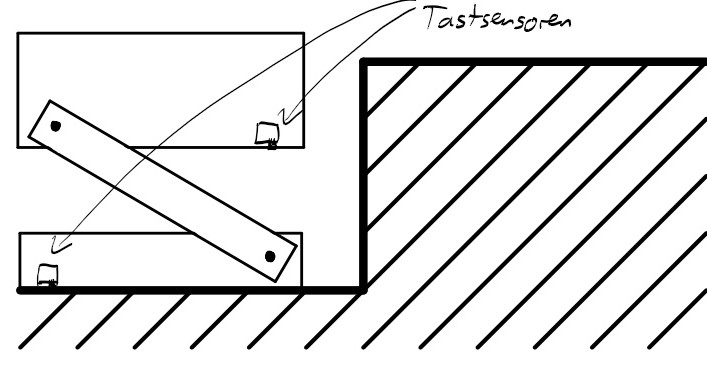
\includegraphics[width=0.6\textwidth]{img/Treppensteigen/Sensoren_Treppensteigen1.png}
  \centering
  \caption{Platzierung der Tastsensoren für die Bewegungen}
  \label{fig2}
\end{figure}

Die Abbildung \ref{fig2} zeigt an welchem Ort der Komponenten die Tastsensoren angebracht werden sollen. Wenn der Roboter sich im Ausgangszustand befindet (eingefahren) sind beide Sensoren aktiv. Danach wird die 1. Hubbewegung so lange ausgeführt bzw. der Motor angesteuert, bis sich der Grundkörper auf der Treppe befindet und der Sensor wieder aktiv ist. Danach wird der zweite Motor für die 2. Hubbewegung solange angesteuert, bis sich die Stützen auf der Treppenstufe befinden bzw. der Sensor wieder aktiv ist.

Bei den Hubbewegungen muss der Grundkörper gerade gehalten werden:
\begin{itemize}
    \item Um in der ersten Hubbewegung der Grundkörper gerade halten zu können, wird ein Drehmoment von 1.2 Nm benötigt. Gemäss Datenblatt des Elektromotors IG320516-41C01 gibt der Motor bei einem Strom von 0.5 A und einer Leistung von 1.51 W ein Drehmoment von 1.31 Nm ab. Daraus folgt eine Spannung von 3V. Diese Spannung kann mit einer H-Brücke eingestellt werden.
    \item Das Prinzip der zweiten Hubbewegung ist analog zur ersten. Der Elektromotor RB350600-0A101R gibt gemäss Datenblatt bei einem Strom von 0.2 A und einer Leistung von 0.51 W ein Drehmoment von 0.6 Nm ab. Daraus folgt eine Spannung von 2.55 V.
 \end{itemize}


\newpage
\subsection{Fortbewegung}
Die horizontale Fortbewegung wird mit zwei, unabhängigen voneinander angetriebenen Rädern ermöglicht. Zusätzlich zu diesen zwei Rädern wird ein Stützrad benötigt, dass der Grundkörper nicht den Boden berührt. Damit das Stützrad beim Treppensteigen kein Hinderniss bei der Hubbewegung ist und nicht an der Kante des nächsten Treppentritts hängen bleibt, soll sich das Stützrad im vorderen Teil des Grundkörpers befinden. 

\image
 {img/Skizze Räder.png}
 {Skizze Räder mit Stützrad}

Dieses Fortbewegungsprinzip ermöglicht es dem Gerät sich an Ort und Stelle zu drehen, indem die Räder entgegegesetzt angesteuert werden. Das Gerät kann sich somit im Start- und Zielbereich in alle Richtungen bewegen. Dies ist zu Beginn, für das Fahren vor die Treppe und zum Schluss, beim Suchen des Zielpiktogramms vorteilhaft. Um auf den Treppenstufen nach links oder rechts auszuweichen, soll sich das Gerät zuerst um 90$^\circ$ drehen, dann geradeaus fahren und sich anschliessend wieder um 90$^\circ$ drehen, sodass sich das Gerät an der Position für den nächsten Treppensteigprozess rechtwinklig vor dem nächsten Treppentritt befindet.

\subsubsection{Berechnung der Antriebsleistung}

Für eine erste Berechnung der notwendigen Antriebsleistung zur Fortbewegung wurde ein Raddurchmesser und eine maximale Wunscheschwindigkeit angenommen. Die Räder sollen aus Gummi sein. Die Materialien, die das Gerät befahren muss sind Holz im Startbereich und Aluminium auf der Treppe. Für die Berechnung des notwendigen Antriebsmoments auf Holz und Aluminium, ohne durchrutschen der Räder, wurde ein Reibungskoeffizent\footnote{https://www.schweizer-fn.de/stoff/reibwerte/reibwerte.php} für die Paarung Gummi-Metall verwendet. Wird das gleiche berechnete Moment auf der Holzunterlage aufgebracht, ist das durchrutschen weniger kritisch, da die Reibung zwischen dem Holz und den Gummirädern grösser ist.

\image
 {img/Radberechnung.png}
 {Skizze zur Radberechnung}\\

\newpage
d$_{Rad}$ = 80 mm

v$_{Wunsch}$ = 2 m/s

{\mu$_{Gummi-Aluminium}$} = 0.5

F$_{Gges}$ = m$_{ges}$ * g = 3 kg * 9.81 m/s$^{2}$ = 29.4 N\\



F$_{N}$ = F$_{Gges}$ / 2 = 29.4 N / 2 = 14.7 N 

F = F$_{R}$ = F$_{N}$ * {\mu$_{Gummi-Aluminium}$} = 14.7 N * 0.5 = 7.35 N\\



M$_{max}$ = F * r = 7.35 N * 0.04 m = 0.3 Nm\\



Kein Rutschen: {\omega$_{max}$} = v$_{Wunsch}$ / r = 2 m/s / 0.04 m = 50 rad/s


\subsubsection{Auswahl der Motoren für die Fortbewegung}

TODO Motorenauswahl

\subsubsection{Überwachung der Fortbewegung}

TODO Sensoren für Überwachung der Fortbewegung

\subsection{Elektrosteuerung}
Die Steuerung der Elektrokomponenten wie Motoren, Sensoren und Kameras erledigen ein Raspberry und ein Arduino Board. Das Raspberry ist dabei in erster Linie für die Bildverarbeitung und das Pathfinding verantwortlich. Dafür wird eine gewisse Rechnerleistung benötigt, welche das Arduino nicht erbringen kann, weshalb ein Raspberry unumgänglich ist.
Auf diesem laufen alle Programme, welche das Vorgehen bestimmen. Diese Befehle werden anschliessend an das Arduino weitergeleitet. Von diesem Board aus werden die Motoren angesteuert und die Sensoren verarbeitet.

\subsubsection{Auslegung Akku}

TODO Stromverbrauch


\subsection{Umgebungserkennung}
\subsubsection{Orientierung}
\textbf{Finden des Piktogramms im Startfeld}\\
Um im Startfeld das Piktogramm zu finden wird die Kamera verwendet. Hier ist geplant, mit einem FindContours-Algorithmus\footnote{https://docs.opencv.org/3.4/df/d0d/tutorial\_find\_contours.html} in OpenCV alle Konturen mit vier Eckpunkten herauszufiltern. Dabei werden diese gefundenen Konturen mit vier Eckpunkten nach der grösse der Fläche sortiert. Dabei wird davon ausgegangen, dass die grösste dieser Konturen das Schild mit dem Piktogramm ist. Es wird angenommen, dass es plausibel ist, dass das grösste Objekt mit genau vier Eckpunkten und Kanten, das Schild mit dem Piktogramm ist.\\ 
Sobald eine plausible Kontur gefunden wurde kann das Bild bereits für die Piktogrammerkennung vorbereitet werden. Hierbei wird es auf die Region of Interes (ROI) begrenzt und optional mit der getGeometricTransform-Methode von OpenCV eine Top-Down-View auf das Bild erstellt. Da es sich bei den Piktogrammen um Schwarz-Weiss-Bilder handelt, kann man hier noch leicht die unterschiedlichen Lichtverhältnisse herausfiltern, in dem man noch eine Threshold anwendet.
Folgend eine Auflistung der geplanten Bildverarbeitungsschritte:
\begin{enumerate}
    \item Verkleinerung
    \item In Graustufen konvertieren 
    \item Verzerren
    \item Erkennen von Kanten (Canny edge detection)
    \item Finden der der Konturen
    \item Sortieren der Konturen nach Fläche
    \item Einzeichnen der Konturen mit grösster Fläche auf dem Originalbild
    \item Auf ROI zuschneiden
    \item Optional: Top-Down-View auf das Bild erstellen (getGeometricTransform())
    \item Thresholding
\end{enumerate}

\textbf{Finden der Treppe im Startfeld}\\
Für das Finden der Treppe soll der gleiche Algorithmus verwendet werden, mit welchem auch das Path-Finding realisiert werden soll. Sobald also das Piktogramm gefunden und der Auftrag quittiert wurde, macht sich der Roboter auf die Suche nach der Treppe. Danach fährt der Roboter an den Start des definierten Pfades. Damit die Ausrichtung zur Treppe genau 90° Beträgt, ist der Roboter mit zwei Tastsensoren an der Vorderseite ausgestattet. Somit kann man einfach solange gegen die Treppe fahren, bis beide Tastsensoren detektieren.

\textbf{Orientierung auf der Treppenstufe}\\
Um sich auf einer Treppenstufe orientieren zu können, ist geplant mithilfe eines Linefollowing Algorithmus der Treppenstufe sicher entlang zu fahren. Ebenfalls ist gedacht, den Linefollowing Algorithmus dazu zu verwenden, die Ausrichtung des Roboters auf der Treppenstufe zu kontrollieren (siehe Kapitel \ref{orientierungAufTreppenstufe}).
Die zurückgelegte Distanz auf einer Treppenstufe soll mithilfe des Encoders der Motoren berechnet werden.

\subsubsection{Hindernisserkennung}

\subsubsection{Piktogrammerkennung}
Erst war geplant, die Piktogrammerkennung mit einem Convolutional Neural Network (CNN) zu realisieren. Hierbei wird ein Modell darauf trainiert, die fünf Piktogramme zu erkennen. Während der Erstellung des Funktionsmusters (siehe Kapitel \ref{piktogrammerkennungMitCNN}) und den Weekly-Standups mit dem Coach hat sich herausgestellt, dass es passendere Techniken gibt.\\
Da es sich um ein endliches Problem handelt, weil man lediglich fünf verschiedene Piktogramme erkennen und unterscheiden muss, war der zweite Lösungsansatz sogenanntes Template Matching\footnote{https://docs.opencv.org/master/d4/dc6/tutorial\_py\_template\_matching.html}. Bei der Recherche hat sich herausgestellt, dass diese Methode gute Resultate liefert, wenn man lediglich mit Translationen und Skalierungen zu tun hat. Sobald das Bild, in dem das Piktogramm detektiert werden soll, Rotationen und nicht affine Transformationen aufweist, ist man besser dran mit Keypoint Detection, Image Deskriptoren und Keypoint Matching\footnote{https://opencv-python-tutroals.readthedocs.io/en/latest/py\_tutorials/py\_feature2d/py\_matcher/py\_matcher.html}. Aus diesem Grund ist geplant die Piktogrammerkennung mit letzterem umzusetzen.




\subsection {Kommunikation}

Um das Finden und Verarbeiten des Piktogramms sowohl im Start- als auch im Zielbereich zuverlässig und einfach zu signalisieren, werden zwei verschiedene Methoden verwendet. Einerseits die Visualisierung mittels LEDs und anderseits die auditive Quittierung. Diese Audiowiedergabe wird entweder mittels Buzzer, oder mittels eines Lautsprechers getätigt. Die Visualisierung mittels LEDs erfolgt über das Raspberry selbst.

Die Audiowiedergabe über den Buzzer ermöglicht einfache Tonabfolgen und wird über die Spannung eines Pins gesteuert. Das Prinzip ist einfach und schnell, ist bezüglich der Lautstärke und dem "WoW-Effekt" dem Lautsprecher jedoch deutlich unterlegen.
Die Ausgabe über die USB-Lautsprecher erfolgt direkt über das Raspberry. Die Speaker werden direkt mittels USB und der 3.5mm Klinke mit dem Raspberry verbunden. Mit wenigen Zeilen Code kann so ein vollwertiges Audiofile abgespielt werden.
Die Lautsprecher sind in jeglicher Hinsicht besser und einfacher mit der Ausnahme des Platzbedarfs. Ist der Platz und das Gewicht verfügbar, werden die Lautsprecher verbaut 

\newpage
\subsection{Zusammenspiel der Teilfunktionen}
 Die Abbildung \ref{fig3} zeigt das Blockschaltbild des Zusammenspiels der Teilfunktionen.

\begin{figure}[h]
  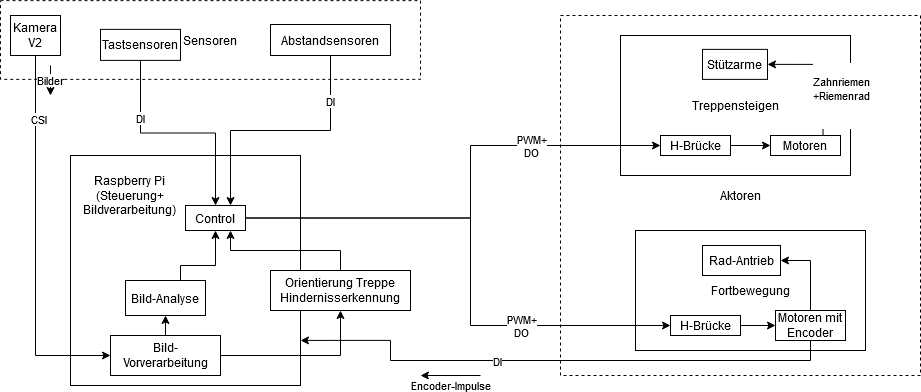
\includegraphics[width=\textwidth]{img/Funktionsmuster Treppensteigen/Blockschaltbild.png}
  \centering
  \caption{Blockschaltbild der Prozesse Elektrotechnik/Mechanik}
  \label{fig3}
\end{figure}

 Das Blockschaltbild zeigt als zentrale Steuerungseinheit einen Raspberry Pi. Dieser übernimmt die Aufgabe der Bildverarbeitung für die Orientierung auf der Treppe sowie für die Hinderniserkennung. Diese Informationen verarbeitet die Steuerung und gibt entsprechende Signale an die Aktoren weiter. Zu den Aktoren gehören die Elektromotoren inkl. H-Brücken für die Ansteuerung, sowie die mechanischen Komponenten für das Treppensteigen und die Fortbewegung. Die Elektromotoren der Fortbewegung senden ein Encodersignal zurück an den Raspberry Pi. Zu den Sensoren des Konzeptes gehören Kameras, die Bilder für die Bildverarbeitung liefern. Zusätzlich liefern Abstands- und Tastsensoren für die Orientierung und das Treppensteigen Inputsignale für die Steuerung.
